\documentclass[a4paper]{article}
\usepackage[pdftex]{graphicx}
\usepackage[utf8]{inputenc}
\usepackage{enumerate}
\usepackage{siunitx}
\sisetup{locale=DE}
\usepackage{icomma}
\usepackage{amssymb}
\usepackage{tikz}
\usepackage{href-ul}
\hypersetup{
	colorlinks=true,
	linkcolor=blue,
	urlcolor=blue}
\usepackage{geometry}
\geometry{a4paper, top=15mm, left=15mm, right=15mm, bottom=15mm,
	headsep=10mm, footskip=12mm}

\begin{document}
	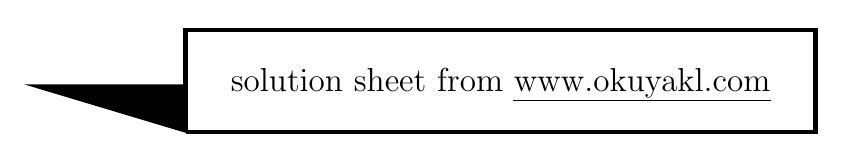
\begin{tikzpicture}(10,3)
		\draw[ultra thick](2,0) --(10,0) -- (10,1.3) --(2,1.3) -- (2,0);
		\draw[fill=black](2,0)-- (0,.6) -- (2,.6) -- (2,0);
		\node at (6,.6) {\large solution sheet from \href{http://www.okuyakl.com}{www.okuyakl.com}};
	\end{tikzpicture}
	\vspace{0.5 cm}
	
	\noindent{\bf Task 1. a)}\\
	The following applies to the Coulomb force between two charged particles:
	$$F_C = {1 \over 4 \pi \varepsilon_0}\cdot {Q_1\cdot Q_2 \over r^2}$$
	We substitute an elementary charge for the charges $Q_1$ and $Q_2$ and get:
	$$F_C = {1 \over 4 \pi \SI{8.85e12}{\ampere\second\over \volt\meter}}\cdot {(\SI{1.60e-19}{\ampere\second} )^2 \over (\SI{5.3e-11}{\meter})^2}=\SI{8.2e-8}{\newton}$$
	Unit check:
	$$\SI{}{(\ampere\second)^2 \over {\ampere\second \over \volt\meter} \cdot m^2}=\SI{}{\ampere\second \cdot \volt\ meter \over \meter^2}= \SI{}{\joule \over \meter} = \SI{}{\newton} $$
	\vspace{0.5 cm}
	
	\noindent{\bf Task 1. b)}\\
	To obtain the gravitational force, we apply the law of gravity and substitute the masses of the proton and electron as well as the gravitational constant G:
	$$ F_G = {G \cdot m_1 \cdot m_2 \over r^2} = { \SI{6.67e-11}{\meter^3 \kilogram^{-1} \second^{-2}} \ cdot\SI{1.67e-27}{\kilogram} \cdot\SI{9.1e-31}{\kilogram} \over (\SI{5.3e-11}{\meter})^2}= \SI{3.6e-47}{\newton}$$
	Unit check:
	$$\SI{}{{\meter^3 \kilogram^{-1} \second^{-2}} \cdot {{\kilogram^2} \over \meter^2}}= \SI{}{ \kilogram \cdot {\meter \over \second^2}} = \SI{}{\newton}$$
	The gravitational force is therefore many orders of magnitude smaller and therefore completely negligible.
	\vspace{0.5 cm}
	
	\noindent{\bf Task 2.}\\
	We equate the gravitational force and the Coulomb force and solve for the charge $Q_2$:
	$$
	\renewcommand{\arraystretch}{2}
	\begin{array}{rcll}
		F_G & = & F_C \\
		{G \cdot m_1 \cdot m_2 \over r^2} & = & {1 \over 4 \pi \varepsilon_0}\cdot {Q_1\cdot Q_2 \over r^2} & | \cdot r^2 \\
		G \cdot m_1 \cdot m_2 & = & {1 \over 4 \pi \varepsilon_0}\cdot Q_1\cdot Q_2 & |\cdot 4 \pi \varepsilon_0 \\
		G \cdot m_1 \cdot m_2 \cdot 4 \pi \varepsilon_0 & = & Q_1\cdot Q_2
		&| : Q_1 \\
		{G \cdot m_1 \cdot m_2 \cdot 4 \pi \varepsilon_0 \over Q_2} & = & Q_1 \\
		Q_1 & = & {\SI{6.67e-11}{\meter^3 \kilogram^{-1} \second^{-2}} \cdot (\SI{1.0e-3}{\kilogram} )^2 \cdot 4 \pi \cdot \SI{8.85e-12}{\ampere\second\over \volt\meter} \over\SI{1.0e-13}{\ampere\second}} & =\SI{7,4e-14}{\ampere\second}
	\end{array}
	$$
	Unit check:
	$$\SI{}{{\meter^3 \kilogram^{-1} \second^{-2}} \cdot \kilogram^2 \cdot {\ampere\second\over \volt\meter} \over \ ampere\second} = \SI{}{\kilogram \cdot {\meter^2 \over \second^2} \over \volt } = \SI{}{\joule \over \volt} = \SI{}{ \volt\cdot \ampere\second \over \volt} = \SI{}{\ampere\second} = \SI{}{\coulomb} $$
	The charge only needs to be the very small value of $\SI{7.4e-14}{\coulomb}$, i.e. $\SI{0.074}{\pico\coulomb}$, which corresponds to about 460,000 electrons.
	\vspace{0.5 cm}
	
	\noindent{\bf Task 3.}\\
	\begin{minipage}{0.6\textwidth}
		We first calculate the angle $\alpha$ from the given geometry:
		$$ \sin \alpha = {0.5\cdot d \over l} \Rightarrow \alpha = \sin^{-1} \left( {\SI{0.2}{\meter} \over \SI{ 1.0}{\meter}} \right)$$
		$$ \alpha = \SI{11,5}{\degree}$$
		This angle occurs once again in the force rectangle below the balls. The following applies to the amounts of the Coulomb force and the weight force:
		$$ \tan{\alpha} = {F_C \over F_G}$$
		This gives us for $F_C$:
		$$F_C = F_G \cdot \tan{\alpha} = \SI{0.05}{\newton} \cdot \tan{\SI{11.5}{\degree}} =
		\SI{0.01}{\newton}$$
	\end{minipage}
	\hspace{1cm}
	\begin{minipage}{0.4\textwidth}
		\includegraphics[width=5 cm]{pelad240.pdf}
	\end{minipage}
	\vspace{0.5 cm}
	
	\noindent Now we solve the formula for the Coulomb force according to the charge and get for $Q_1=Q_2=Q$:
	$$
	\renewcommand{\arraystretch}{2}
	\begin{array}{rcll}
		F_C & = & {1 \over 4 \pi \varepsilon_0}\cdot {Q^2 \over d^2} & | \cdot r^2 \cdot 4 \pi \varepsilon_0 \\
		F_C \cdot 4 \pi \varepsilon_0 \cdot d^2 & = & Q^2 & | \sqrt{\quad}\\
		\sqrt{F_C \cdot 4 \pi \varepsilon_0}\cdot d & = & Q \\
		Q & = & \sqrt{\SI{0.01}{\newton} \cdot 4 \pi \cdot\SI{8.85e-12}{\ampere\second \over \volt\meter}} \cdot \SI{0,4}{\meter} \\
		Q & = & \SI{4e-7}{\coulomb}
	\end{array}
	$$
	Unit check:
	$$\sqrt{\SI{}{\newton \cdot {\ampere\second\over \volt\meter}}} \cdot \SI{}{\meter} = \sqrt{\SI{}{{\joule \over \meter} \cdot {\coulomb \over \joule \cdot \coulomb^{-1}\cdot \meter}}} \cdot \SI{}{\meter} = \sqrt{ \SI{}{{ \coulomb^2} \over {\meter^2}}} \cdot \SI{}{\meter} = \SI{}{\coulomb}$$
	The amount of the load on the Kugeln is $0.4\SI{}{\micro \coulomb}$
	\vspace{0.5 cm}
	
	\noindent{\bf Task 4. a)}\\
	The magnitude of the electric field strength at a point at a distance $r$ from the center of the sphere is:
	$$ E = {1 \over 4 \pi \varepsilon_0}\cdot {Q \over r^2} =
	{1 \over 4 \pi \SI{8.85e-12}{\ampere\second\over \volt\meter}}\cdot {\SI{1e-9}{\ampere\second} \over r^2 }= \SI{9,0}{\volt\meter} \cdot{1 \over r^2} \qquad (*)$$
	\vspace{0.5 cm}
	
	\noindent{\bf Task 4. b)}\\
	For $r$ we insert once $R=\SI{4,5}{\centi\meter}$ and once $3R=\SI{13,5}{\centi\meter}$ in $(*)$ and receive:
	$$ E_R = {\SI{9}{\volt\meter} \over (\SI{0.045}{\meter})^2}= \SI{4.4}{\kilo\volt\over\meter} $$
	$$ E_{3R} = {\SI{9}{\volt\meter} \over (\SI{0.135}{\meter})^2}= \SI{0.49}{\kilo\volt\over \meter}$$
	So the field strength is in the range $\SI{4.4}{\kilo\volt\over\meter} > E > \SI{0.49}{\kilo\volt\over\meter}$
	\vspace{1cm}
	
	\begin{minipage}{0.5\textwidth}
		\noindent{\bf Task 4. c)}\\
		\includegraphics[width=8 cm]{kufeld240.pdf}
	\end{minipage}
	\begin{minipage}{0.45\textwidth}
		\noindent{\bf Task 4. d)}\\
		Inside the sphere the field strength is zero; see vertical line.
		
		\noindent{\bf Task 4. e)}\\
		It applies to the Coulomb force on the test charge $q$
		$$F_C=q \cdot E $$
		Here $q=2\cdot e$ is the charge of the $\alpha$ particle and $E$ is the field strength at a distance of 13.5 cm:
		$$F_C= 2\cdot\SI{1.60e-19}{\coulomb} \cdot \SI{490}{\volt\over\meter}=\SI{1.6e-16}{\newton}$$
		Unit check:
		$$ \SI{}{\coulomb \cdot {\volt\over \meter}} = \SI{}{\coulomb \cdot {\joule \over \coulomb\cdot \meter}} = \SI{}{{ \newton \meter \over \meter}} = \SI{}{\newton}$$
	\end{minipage}
	\vspace{0.5 cm}
	
	\noindent The force on the helium nucleus is directed away from the sphere because both bodies are positively charged.
	\vspace{0.5 cm}
	
	\noindent{\bf Task 5. a)}\\
	We solve $(*)$ from problem 4. a) for $Q$:
	$$
	\renewcommand{\arraystretch}{2}
	\begin{array}{rcll}
		E_1 & = & {1 \over 4 \pi \varepsilon_0}\cdot {Q \over d^2} &|\cdot d^2 \cdot 4 \pi \varepsilon_0 \\
		E_1 \cdot d^2 \cdot 4 \pi \varepsilon_0 & = & Q \\
		Q & = & \SI{100}{\volt\over \meter} \cdot (\SI{0.525}{\meter})^2\cdot 4 \pi \cdot\SI{8.85e-12}{\ coulomb \over \volt\meter} &= \SI{3,1e-9}{\coulomb}
	\end{array}
	$$
	Unit check:
	$$ \SI{}{{\volt\over \meter} \cdot \meter^2 \cdot {\coulomb \over \volt\meter}} = \SI{}{\coulomb}$$
	\vspace{0.5 cm}
	
	\noindent{\bf Task 5. b)}\\
	The radius of the charged balloon plays no role in the field strength outside the balloon. The field strength at the distance $d>r_2$ behaves as if the entire charge were concentrated at the center of the balloon.
	\vspace{0.5 cm}
	
	\noindent{\bf Task 6.}\\
	
	\begin{minipage}{0.3\textwidth}
		The following applies to the distance $a$ of the field-free point $P$ from the charge $Q_2$:
		$$ a= d-s \quad (**)$$
	\end{minipage}
	\begin{minipage}{0.65\textwidth}
		\includegraphics[width=10 cm]{fefrei240.pdf}
	\end{minipage}
	\vspace{0.5 cm}
	
	\noindent We use $(*)$ again, this time on the right and left, because in the field-free point both field strengths cancel each other out; Here they are equal in amount and opposite in direction:
	$$
	\renewcommand{\arraystretch}{2}
	\begin{array}{rcll}
		E_1 & = & E_2 \\
		{1 \over 4 \pi \varepsilon_0}\cdot {Q_1 \over s^2} & = & {1 \over 4 \pi \varepsilon_0}\cdot {Q_2 \over a^2} &| \cdot 4 \pi \varepsilon_0 \\
		{ Q_1 \over s^2} & = & {Q_2 \over a^2} & | : Q_1 \cdot a^2 \\
		{ a^2 \over s^2} & = & {Q_2 \over Q_1} & | \sqrt{\quad} \\
		{ a \over s} & = & \sqrt{Q_2 \over Q_1} &| (**)\\
		{ d-s \over s} & = & \sqrt{Q_2 \over Q_1} \\
		{d \over s}-1 & = & \sqrt{Q_2 \over Q_1} &|+1 \quad |\cdot s\\
		d & = & s \cdot \left( \sqrt{Q_2 \over Q_1}+1 \right)\\
		d & = & \SI{0,1}{\meter} \cdot \left( \sqrt{\SI{5,5}{\nano\coulomb} \over \SI{8,5}{\nano\coulomb }}+1 \right) &=
		\SI{0.18}{\meter}
	\end{array}
	$$
	The distance between the two point charges is 18 cm.
	
	\begin{center}
		\includegraphics[width=7 cm]{../../viecher/eendcomic.pdf}
		
		Here you can go back to the \href{https://www.okuyakl.de/phys/p11coulL240/ae240.pdf}{task sheet}
	\end{center}
	
	\end{document}